\section{Goldstone's theorem}

\begin{figure}[ht]
    \centering
    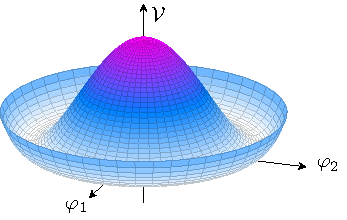
\includegraphics[]{figurer/mexican_hat.pdf}
    \caption{The Mexican hat potential.}
    \label{fig:Mexican hat}
\end{figure}


The ground state of a theory is not necessarily invariant under the symmetry transformations of the theory.
This is exemplified by the linear sigma model,
\begin{equation}
    \Ell[\varphi] 
    = \frac{1}{2} \partial_\mu \varphi_i(x) \partial^\mu \varphi_i(x) - \Ve(\varphi),
    \quad \Ve(\varphi) = - \frac{1}{2} \mu^2 \varphi_i(x)\varphi_i(x)
    + \frac{1}{4} \lambda [\varphi_i(x) \varphi_i(x)]^2.
\end{equation}
The linear sigma model Lagrangian is invariant under the rotation of the $N$ fields,
\begin{equation}
    \varphi_i \longrightarrow \varphi_i' = O_{ij} \varphi_j,
    \quad O^{-1} = O^{T}.
\end{equation}
This is a global, internal and continuous set of transformations, with the infinitesimal form
\begin{equation}
    \varphi_i(x) = \varphi_i(x) + \epsilon \, i t_{ij} \varphi_j(x)
\end{equation}
The group of all such transformations form the Lie group $O(N)$. (SKRIVE APPENDIX OM LIE GRUPPER?)
If we assume the ground state $\varphi_{0}$ is translationally invariant, then it is given by minimizing the effective potential.
The first approximation of this is given by the classical potential, $\Ve$.
For $N=2$, this is the famous ``Mexican hat''-potential, as illustrated by \autoref{fig:Mexican hat}.
The ground state is therefore given by any of the values along the brim of the potential.
If we, without loss of generality, choose $\varphi = (0, v)$ as the ground state, then any symmetry transformation will change this state.
We say that the symmetry has been \emph{spontaneously broken}.
We can express this mathematically as
\begin{equation}
    t_{ij} \ex{ \varphi_i}_0 \neq 0.
\end{equation}

If we take the constraint \cref{effective equation of motion}, differentiate with respect to $\varphi_j(y)$ and evaluate in the vacuum, we get
\begin{equation}
    \int \dd^4 x \, \fdiff{\Gamma[\varphi_0]}{\varphi_j(y), \varphi_i(x)}
    t_{ik} \ex{\varphi_k}_0 = 0.
\end{equation}
In \autoref{Effective action inverse propagator}, we found that the second derivative of the effective action is the inverse propagator.
The momentum space propagator is therefore
\begin{equation}
    i \delta(0) \tilde D_{ji}^{-1}(p) 
    = \int \dd^4 x \, e^{-i p x}  
    \fdiff{\Gamma[\varphi_0]}{\varphi_j(0), \varphi_i(x)}.
\end{equation}
(CHECK THAT)
If we assume the ground state is independent of space-time, we get
\begin{equation}
    \tilde D^{-1}_{i j}(p=0) \, t_{j k} \ex{\varphi_k}_0 
    = \diffp{\Veff}{\varphi_i, \varphi_j} \, t_{j k} \ex{\varphi_k}_0  
    = 0.
\end{equation}
If the symmetry transformation $\varphi_i \rightarrow \varphi_i + i \epsilon t_{ij} \varphi_j$ remains unbroken, then this is trivial, as $t_{ij} \ex{\varphi_j }_0= 0$.
However, if it is a broken symmetry, then by definition $t_{ij} \ex{\varphi_j }_0 \neq 0$.
In that case, $t_{ij} \ex{\varphi_j}_0$ has a zero eigenvalue of the inverse propagator, at $p = 0$.
In other words, the system contains a zero-mass particle, a Goldstone boson.\footnote{ The particles are bosons due to the bosonic nature of the transformations, $t$. If the generators are Grassmann numbers, the resulting particle, called a goldstinos, are fermions.}

The set of continuous symmetry transformations, 
\begin{equation}
    G = \setbuilder{g}{g \varphi = \varphi', \, S[\varphi'] = S[\varphi], \D \varphi' = \D \varphi },
\end{equation}
form a Lie group.
This is a manifold, i.e. a space that is local homeomorphic to $\R^N$, and thus can be parametrized by $N$ real numbers $\eta_\alpha$, while also having a group structure, composition of transformations.
We will focus on connected Lie groups, in which we all elements $g \in G$ is in the same connected piece as the identity map $\id(\varphi) = \varphi$.
This means that for each $g\in G$, one can find a continuous path $\gamma(t)$ in the manifold, such that $\gamma(0) = \id$ and $\gamma(1) = g$.
Given such a path, we can study transformations close to the identity.
As the Lie group is a smooth manifold, we can write
\begin{equation}
    \gamma(\epsilon) = \id + i \epsilon V + \Oh{\epsilon}.
\end{equation}
$V$ is a generator, and is a part of the tangent space of the identity element, $T_\id$.\footnote{The factor $i$ is a physics convention, and differs from how mathematicians define generators of a lie group.}
The set of generators such $T_\id$, thus forms a vector space, and the coordinates $\eta_a$ induce a coordinate basis.
This can be written as a path through parameter space, $\gamma(t) = g(\eta(t))$, which gives
\begin{equation}
    V = \diff{\gamma}{t}\Big|_{t=0} = \diff{\eta_a}{t}\Big|_{t=0} \diffp{g}{\eta_a}\Big|_{\eta=0}.
\end{equation}
The parameters therefore gives a basis for $T_\id$, and we can write
\begin{equation}
    \gamma(\epsilon) = \id + i \epsilon v_\alpha T_\alpha + \Oh{\epsilon}, 
    \quad 
    T_\alpha = \diffp{g}{\eta_\alpha}.
\end{equation}
% TODO:?? Skrive om structure constants
% \end{equation}
% Furthermore, using the group structure of $G$ we can write
% \begin{equation}
%     g(\eta) g(\eta') = g(f(\eta, \eta')).
% \end{equation}
% If we assume $g(\eta=0) = \id$, then we must have $f_a(\eta, 0) = f_a(0, \eta) = \eta_a$.
% This allows us to write
% \begin{equation}
%     f_a(\eta, \eta') = \eta_a
% \end{equation}
% The taylor expansion of this function is therefore
% \begin{equation}
%     f_a(\eta, \eta') = \eta_a + \eta_a' + f_a^{bc}\eta_b \eta_c'
% \end{equation}
The tangent space, together with the additional operation
\begin{align}
    [T_\alpha, T_\beta] = iC_{\alpha\beta}^\gamma T_\gamma,
\end{align}
called the Lie bracket, forms a Lie algebra.
For matrix groups, which are what we deal with in this text, the Lie bracket is the commutator.
$C_{\alpha \beta}^\gamma$ are called the structure constants, and are totally antisymmetric.
This is equivalent with them obeying the Jacobi identity,
\begin{equation}
    \label{jacobi identity}
    C_{\alpha \beta\gamma} + C_{\beta\gamma\alpha} +  C_{\gamma\alpha\beta} = 0.
\end{equation}
The exponential maps elements of the Lie algebra to the Lie group.
In fact, every element of the Lie group can be written
\begin{equation}
    g(\eta) = \exp{i \eta_\alpha T_\alpha}.
\end{equation}
For matrix group, the exponential is defined by its series expansion,
\begin{equation}
    \exp(X) = \sum_n \frac{1}{n!} X^n.
\end{equation}

A subset of the original Lie group, $H \subset G$, which is closed under the group action is called a subgroup.
In the case of symmetry breaking, a subset of the original generators, $x_i$, where $i \in \{1,... m\}$ may correspond to a symmetry of the ground state.
That is,
\begin{equation}
    x_i \varphi_0 = 0.
\end{equation}
The group elements of $G$ that has the form $h = \exp{i \xi_i x_i}$ form a subgroup $H$, with dimension $m = \dim H$.
The set of generators $t_a$, on the other hand, do not form a subgroup, as the identity transformation $\id$ is a part of $H$.
These are called \emph{Broken generators}.
As the union of $x_i$ and $t_a$ make up the total set of original generators, $T_\alpha$, the number of broken generators are $n_G = \dim G - \dim H$
In Lorentz invariant systems this corresponds to one massless mode per broken generator, so there are a total of $n_G$ Goldstone bosons.
As a subgroup $H$ of a Lie group $G$ is a Lie group in its own right, the generators of the subgroup forms a closed algebra.
We can write the commutators as 
\begin{align}
    [x_i, x_j] &= i C_{i j}^{k} x_k,\\
    [x_i, t_a] &= i C_{i a}^b t_b, \\
    [t_a, t_b] &= i C_{ab}^k x_k + i C_{ab}^c t_c,
\end{align}
where $ijk$ runs over the unbroken generators, and $abc$ runs over the broken.
The second formula can be derived using the Jacobi identity \cref{jacobi identity}, which implies that $C_{ia}^k = -C_{ik}^a = 0$.


\begin{figure}[ht]
    \centering
    \begin{subfigure}{0.54\textwidth}
        \centering
        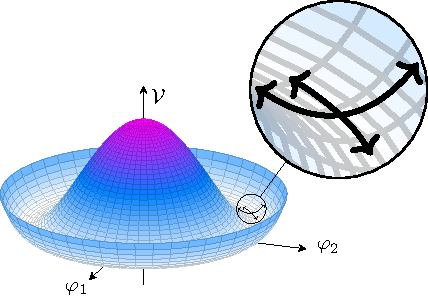
\includegraphics[]{figurer/mexican_hat_zoom.pdf}
        \caption{Excitations along the brim does not cost any energy.}
        \label{fig:Mexican hat zoom}
    \end{subfigure}
    \begin{subfigure}{0.45\textwidth}
        \centering
        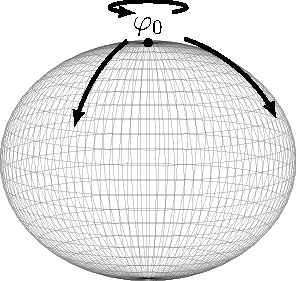
\includegraphics[]{figurer/sigma_ground_state.pdf}
        \caption{Excitations for the $N=3$ sigma model. Two of the symmetries are broken, while rotations around the groundstate leaves the system unchanged.}
        \label{fig:ground state manifold}
    \end{subfigure}
\end{figure}

The Mexican hat potential gives an intuition for the Goldstone mode.
In the case of the two-dimensional sigma model, the symmetry of the Lagrangian are rotations in the plane.
As the ground stat is along the ``brim'' of the hat, this rotational symmetry is broken.
Any excitations in this direction, however, does not cost any energy, which is indicative of a massless mode.
This is illustrated in \autoref{fig:Mexican hat zoom}.
In this example, the original symmetry group is one dimensional, so there is no unbroken symmetries.
If we instead consider the three-dimensional linear sigma model, which has a three-dimensional symmetry group, rotations of the sphere.
The ground state manifold, the set of all the degenerate ground states, is then a sphere.
When the system chooses one single ground state, this symmetry is broken, but only for two of the generators. 
The generator for rotations around the ground state leaves the that point unchanged, and is thus an unbroken symmetry.
This is illustrated in \autoref{fig:ground state manifold}.

